\documentclass[11pt,a4paper]{article}
\usepackage[margin=22mm,headheight=15pt]{geometry}
\usepackage[T1]{fontenc}
\usepackage{lmodern,amsmath,amssymb,booktabs,tabularx,array,xcolor,tikz,fancyhdr}
\usetikzlibrary{arrows.meta,positioning}
\usepackage[unicode,colorlinks=true,linkcolor=teal!65!black,urlcolor=teal!65!black,citecolor=teal!65!black]{hyperref}
\definecolor{ink}{HTML}{193943}
\definecolor{accent}{HTML}{116D61}
\definecolor{mist}{HTML}{EAF3EF}
\hypersetup{
  pdftitle={Biomass Supply Chain Planning via Mixed-Integer Linear Programming: Mathematical Formulation, Verification, and Scenario Analysis},
  pdfauthor={Mohamad Jamalzehi, Kosar Ghazali},
  pdfsubject={A reproducible research manuscript on biomass district heat supply},
  pdfkeywords={biomass, district heating, MILP, verification, inventory, HiGHS}
}
\newcommand{\repo}{https://github.com/mohammad-jamalzehi/Bio-Mass-Supply-Chain}
\newcolumntype{Y}{>{\raggedright\arraybackslash}X}
\setlength{\parindent}{0pt}
\setlength{\parskip}{4pt}
\setlength{\textfloatsep}{14pt plus 2pt minus 2pt}
\setlength{\intextsep}{10pt plus 2pt minus 2pt}
\setlength{\emergencystretch}{2em}
\renewcommand{\topfraction}{.9}
\renewcommand{\textfraction}{.08}
\renewcommand{\floatpagefraction}{.78}
\setlength{\tabcolsep}{5pt}
\renewcommand{\arraystretch}{1.11}
\pagestyle{fancy}
\fancyhf{}
\fancyhead[L]{\small\color{ink} Biomass supply chain planning}
\fancyhead[R]{\small Mohamad Jamalzehi and Kosar Ghazali}
\fancyfoot[R]{\small\thepage}
\renewcommand{\headrulewidth}{0.35pt}

\newsavebox{\commandsbox}
\begin{document}
\hypersetup{pageanchor=false}
\begin{titlepage}
\thispagestyle{empty}
\vspace*{12mm}
{\color{accent}\large\bfseries RESEARCH CASE STUDY\par}
\vspace{8mm}
{\color{ink}\LARGE\bfseries\raggedright
Biomass Supply Chain Planning via\\
Mixed-Integer Linear Programming:\\
Mathematical Formulation, Verification,\\
and Scenario Analysis\par}
\vspace{7mm}
{\large Mohamad Jamalzehi \\[2pt] Kosar Ghazali\par}
\vspace{12mm}
{\color{accent}\rule{\textwidth}{1pt}}
\vspace{4mm}
{\large\bfseries Abstract\par}
This case study formulates daily procurement, inventory and heat dispatch for
a biomass district-heating network as a mixed-integer linear program. It
compares an archived GAMS formulation with a separately implemented Python
model that conserves each fuel, consistently converts volume to useful heat,
and accounts for natural-gas emissions once per day. Independently enumerated
synthetic tests certify costs of 33.00 for a one-fuel fixture and 5.00, 8.40, and
10.00 for three two-plant fixtures. Historical-input experiments over three and
seven days reached solver optimality. Three 365-day searches reached their
30-second limits with independently audited feasible plans and reported gaps
of approximately 0.011--0.029\%. These annual experiments assess feasibility
under stated assumptions. Demand, plant capacity interpretation and emissions
factor accuracy remain unresolved.
\vspace{6mm}

\textbf{Keywords.} Biomass logistics, district heating, mixed-integer linear
programming, inventory conservation, model verification, scenario analysis.

\vfill
{\small\textbf{Research artifacts}\quad \href{\repo}{\nolinkurl{github.com/mohammad-jamalzehi/Bio-Mass-Supply-Chain}}\par}
\end{titlepage}
\hypersetup{pageanchor=true}

\section{Introduction and motivation}
A campus district-heating operator must meet daily useful-heat demand while
scheduling discrete deliveries, using limited storage and allocating feedstocks
among conversion plants. Natural gas backs up biomass when material or plant
capacity is insufficient. This study asks whether a corrected, auditable model
can reproduce hand-solvable cases and what the archived inputs support at a
longer horizon. The contributions are the explicit formulation, independently
checked synthetic fixtures, and reproducible, qualified annual diagnostics.

\section{Related literature and provenance}
Malladi and Sowlati \cite{malladi2020} examine biomass district heating under
carbon pricing and calculate cost--emissions trade-offs. This is a verified
related publication. The repository's archived report \cite{historicalreport}
shares its title and discusses a UBC district-heating case. The archive has
no formal bibliography and refers to an unnamed article. Its exact
relationship to Malladi and Sowlati's publication has not been independently
established. Their policy conclusions and trade-off results are outside the
numerical claims of this manuscript. For future work, the augmented epsilon-constraint method offers a
systematic approach to generating efficient solutions \cite{mavrotas2009}.
The equations and validation experiments below document this project's Python
implementation. They are derived from the physical accounting described here,
rather than transcribed as a reproduction of the published policy model.

\section{Problem description and system boundary}
Three feedstocks arrive by full truck: wood chips, wood pellets and briquettes.
Fresh material may be burned immediately or retained. Previously stored fuel
may supply either biomass plant. Existing and new units deliver useful heat,
supplemented by gas. The facilities are fixed. The model uses deterministic
daily inputs, constant fuel properties, lossless inventories and end-of-day
storage limits. It excludes supplier locations, route choice, receiving-time
peak stock, investment, explicit freight charges, carbon pricing, and lifecycle
inventory. Figure~\ref{fig:network} distinguishes material and heat connections.

\begin{figure}[htbp]
\centering
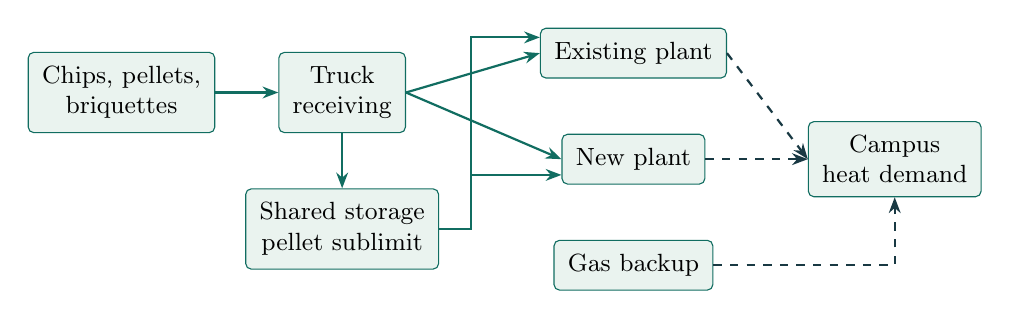
\begin{tikzpicture}[node distance=7mm and 8mm, every node/.style={font=\small},
  box/.style={draw=accent,rounded corners=2pt,fill=mist,align=center,inner sep=5pt},
  material/.style={-{Stealth[length=2mm]},draw=accent,thick},
  heat/.style={-{Stealth[length=2mm]},draw=ink,thick,dashed}]
\node[box] (fuels) {Chips, pellets,\\ briquettes};
\node[box,right=of fuels] (receive) {Truck\\ receiving};
\node[box,below=of receive] (stock) {Shared storage\\ pellet sublimit};
\node[box,right=17mm of receive,yshift=5mm] (old) {Existing plant};
\node[box,below=of old] (new) {New plant};
\node[box,below=of new] (gas) {Gas backup};
\node[box,right=13mm of new] (load) {Campus\\ heat demand};
\draw[material] (fuels)--(receive);
\draw[material] (receive)--(stock);
\draw[material] (receive.east)--(old.west);
\draw[material] (receive.east)--(new.west);
\draw[material] (stock.east)--++(4mm,0) |- ([yshift=2mm]old.west);
\draw[material] (stock.east)--++(4mm,0) |- ([yshift=-2mm]new.west);
\draw[heat] (old.east)--(load.west);
\draw[heat] (new.east)--(load.west);
\draw[heat] (gas.east)-|(load.south);
\end{tikzpicture}
\caption{Planning topology. Solid links carry material volume (\(\mathrm{m^3}\));
dashed links carry useful heat (GJ).}
\label{fig:network}
\end{figure}

\section{Corrected mathematical formulation}\label{sec:math}
Let \(f\in\mathcal F=\{\mathrm{wc},\mathrm{wp},\mathrm{bq}\}\),
\(p\in\mathcal P=\{\mathrm{existing},\mathrm{new}\}\), and
\(t\in\{1,\ldots,T\}\). The one-fuel model is the singleton special case.
Tables~\ref{tab:params} and \ref{tab:vars} define the notation.

\begin{table}[htbp]
\small
\caption{Input parameters and derived heat coefficient.}
\label{tab:params}
\begin{tabularx}{\textwidth}{@{}llY@{}}
\toprule Symbol & Unit & Meaning \\ \midrule
\(V_f,\rho_f\) & \(\mathrm{m^3/truck}\), wet \(\mathrm{t/m^3}\) & Full-truck volume and wet density.\\
\(m_f,h_f\) & fraction, \(\mathrm{GJ/dry\ t}\) & Wet-basis moisture and dry heating value.\\
\(\eta_{pf},q_{pf}\) & fraction, \(\mathrm{GJ/m^3}\) & Plant efficiency and derived useful heat coefficient.\\
\(c_f,c_g\) & source currency/dry t, /GJ & Fuel purchase price and price of useful gas heat.\\
\(e_{pf},e_g\) & \(\mathrm{tCO_2e/GJ}\) & Accounting factors per useful GJ.\\
\(D_t,L_t,K_{pt}\) & GJ, trucks, GJ & Daily demand, shared truck cap and plant heat cap.\\
\(S_t,S^{wp}_t\) & \(\mathrm{m^3}\) & Shared closing storage and optional pellet sublimit.\\
\(I_f^0,I_f^T,\bar G_t\) & \(\mathrm{m^3},\mathrm{m^3},\mathrm{GJ}\) & Opening stock, optional terminal target and optional gas cap.\\
\bottomrule
\end{tabularx}
\end{table}
\begin{table}[htbp]
\small
\caption{Decisions and derived quantities.}
\label{tab:vars}
\begin{tabularx}{\textwidth}{@{}llY@{}}
\toprule Symbol & Domain or unit & Meaning\\ \midrule
\(N_{ft}\) & Nonnegative integer, trucks & Full truckloads received.\\
\(F_{fpt},U_{fpt}\) & Nonnegative real, \(\mathrm{m^3}\) & Fresh and stored biomass burned.\\
\(I_{ft}\) & Nonnegative real, \(\mathrm{m^3}\) & Closing inventory.\\
\(G_t\) & Nonnegative real, GJ & Useful gas heat.\\
\(A_{ft},O_{ft},H_{fpt}\) & Derived, \(\mathrm{m^3},\mathrm{m^3},\mathrm{GJ}\) & Delivery volume, opening volume and useful biomass heat.\\
\bottomrule
\end{tabularx}
\end{table}

\subsection{Heat, procurement cost and emissions accounting}
All volume flows are measured on the delivered basis; useful heat is measured
after conversion. Density converts volume to wet mass and \(1-m_f\) converts
wet to dry mass:
\begin{equation}\label{eq:coefficient}
q_{pf}=\rho_f(1-m_f)h_f\eta_{pf}.
\end{equation}
Both burn streams share a conversion coefficient for a given fuel and plant:
\begin{equation}\label{eq:delivery}
A_{ft}=V_fN_{ft},\qquad H_{fpt}=q_{pf}(F_{fpt}+U_{fpt}).
\end{equation}
The implemented optimization pays for delivered dry fuel and useful gas heat:
\begin{equation}\label{eq:cost}
\min \sum_{t,f}c_f\rho_f(1-m_f)A_{ft}+\sum_t c_gG_t.
\end{equation}
Opening inventory incurs no purchase charge in this window. Emissions are
evaluated afterward and do not influence dispatch:
\begin{equation}\label{eq:emissions}
E=\sum_{t,p,f} e_{pf}H_{fpt}+\sum_t e_gG_t .
\end{equation}
The gas contribution occurs once per day. Factors are provisional in the
historical-input experiments.

\subsection{Availability, conservation and operating constraints}
Plants share available stocks. Each draw is summed across plants:
\begin{equation}\label{eq:avail}
\sum_p F_{fpt}\le A_{ft},\qquad \sum_p U_{fpt}\le O_{ft}\quad(\forall f,t).
\end{equation}
Daily volume is conserved without disposal or storage loss:
\begin{equation}\label{eq:stock}
I_{ft}=O_{ft}+A_{ft}-\sum_p(F_{fpt}+U_{fpt})\quad(\forall f,t).
\end{equation}
Opening stock and any final target are stated explicitly:
\begin{equation}\label{eq:boundary}
\begin{aligned}
O_{f1}&=I_f^0,\qquad O_{ft}=I_{f,t-1}\quad(t>1),\\
I_{fT}&=I_f^T\quad\text{if specified}.
\end{aligned}
\end{equation}
All feedstocks compete for the same daily truck allowance:
\begin{equation}\label{eq:trucks}
\sum_f N_{ft}\le L_t\quad(\forall t).
\end{equation}
The optional silo limit is a pellet-only sublimit within shared closing storage:
\begin{equation}\label{eq:storage}
\sum_f I_{ft}\le S_t,\qquad I_{\mathrm{wp},t}\le S^{wp}_t\quad\text{if specified}.
\end{equation}
The model limits each plant and meets campus demand exactly:
\begin{equation}\label{eq:plant}
\sum_f H_{fpt}\le K_{pt}\quad(\forall p,t).
\end{equation}
\begin{equation}\label{eq:demand}
\sum_{p,f}H_{fpt}+G_t=D_t\quad(\forall t).
\end{equation}
Gas supply is capped only when a cap is provided:
\begin{equation}\label{eq:gas}
G_t\le\bar G_t\quad\text{if specified}.
\end{equation}
Only the truck variables are constrained to integer values:
\begin{equation}\label{eq:domains}
N_{ft}\in\mathbb Z_{\ge0},\qquad F_{fpt},U_{fpt},I_{ft},G_t\in\mathbb R_{\ge0}.
\end{equation}
Constants multiply decision variables throughout \eqref{eq:cost}--\eqref{eq:domains}.

\section{Original GAMS model versus corrected Python MILP}
The archived code \cite{historicalgams} solves distinct problems for
purchase cost \(z_1\) and modeled emissions \(z_2\), both with CPLEX. Each
solve includes only its own objective equation. The final display can therefore
retain a cost level from one solution while the dispatch comes from another.
This is not a cost--emissions trade-off study. Table~\ref{tab:contrast}
summarizes the corrections and refers to the implemented equations.

\begin{table}[htbp]
\small
\caption{Separation of the archived formulation from the Python model.}
\label{tab:contrast}
\begin{tabularx}{\textwidth}{@{}lYY@{}}
\toprule Issue & Original GAMS & Corrected Python\\ \midrule
Material & \texttt{co3} and \texttt{co4} force zero prior closing volume;
\texttt{co2} links stored burn to current closing. & Separate opening and
fresh availability, conserved stocks \eqref{eq:avail}--\eqref{eq:boundary}.\\
Useful heat & Density omitted for fresh fuel in the existing unit's demand term.
& Same dimensional conversion in plant limits and demand \eqref{eq:coefficient}, \eqref{eq:demand}.\\
Emissions & Gas term appears inside a sum over days and fuels. & One gas
term per day, evaluated after dispatch \eqref{eq:emissions}.\\
Silo & \texttt{co7} caps every fuel at the stated pellet-silo volume. &
Optional pellet-only sublimit within total closing volume \eqref{eq:storage}.\\
\bottomrule
\end{tabularx}
\end{table}

\section{Input data and interpretation}
Table~\ref{tab:fuels} transcribes values shared by the GAMS source and
archived report Tables 2--5 \cite{historicalgams,historicalreport}.
Table~\ref{tab:historical} records uncertainty. Agreement on transcription
does not confirm site measurements. The Phase 2 and Phase 3 test fixtures
are wholly synthetic.

\begin{table}[htbp]
\small
\caption{Historical fuel inputs. Costs are in source dollars per dry tonne;
density is wet tonnes per cubic metre and heating value is GJ per dry tonne.}
\label{tab:fuels}
\begin{tabularx}{\textwidth}{@{}Yrrrrrr@{}}
\toprule Fuel & Cost & Density & Moisture & Heating value & Existing & New\\ \midrule
Wood chips & 20 & 0.15 & 0.30 & 12.5 & 0.735 & 0.768\\
Wood pellets & 90 & 0.75 & 0.10 & 18 & 0.763 & 0.811\\
Briquettes & 136 & 1.20 & 0.12 & 19 & 0.761 & 0.807\\
\bottomrule
\end{tabularx}
\end{table}
\begin{table}[htbp]
\small
\caption{Historical inputs and scenario-specific interpretations.}
\label{tab:historical}
\begin{tabularx}{\textwidth}{@{}lYY@{}}
\toprule Input & Archived evidence & Treatment in the experiments\\ \midrule
Demand & GAMS: 12,624 GJ/day for 365 days; no matching value identified in report. &
Retained in all named variants; approximately 146 MW average, unconfirmed.\\
Receiving and storage & Six trucks/day of 110 \(\mathrm{m^3}\) each;
412 \(\mathrm{m^3}\) shared total and 192 \(\mathrm{m^3}\) silo. &
Full trucks; silo inside shared end-of-day storage. Site arrangement unconfirmed.\\
Existing plant & 518.4 GJ/day; 6 MW in report narrative. & Retained; 24-hour availability implicit in conversion.\\
New plant & 1,555.2 GJ/day in model and report table; 12 MW addition and 18 MW combined in narrative. &
Baseline 1,555.2 GJ/day; narrative alternative 1,036.8 GJ/day.\\
Gas & 37 source dollars per useful GJ; capacity unspecified. & Uncapped.\\
Emissions & GAMS 0.96/0.5 wood/gas; report 0.094/0.056. & Separate factor scenario,
used provisionally per useful GJ; accounting boundary unresolved.\\
Inventory & No dependable opening or final stock targets. & Both explicitly set to zero for these experiments.\\
\bottomrule
\end{tabularx}
\end{table}

\section{Optimization and independent verification}
SciPy \cite{scipy2020} passes a sparse MILP to HiGHS via \texttt{milp}
\cite{scipymilp,huangfu2018}. Each column represents a decision; each row
enforces a bounded linear expression. The annual records identify SciPy
1.18.1 and HiGHS 1.12.0. The annual adapter adds a time limit while
retaining the original Phase 3 model and rescales costs to thousands of
source dollars for numerical summation. Costs in this paper are converted
back to their original denomination.

The independent audit reconstructs per-fuel ledgers and per-plant useful heat,
recomputes procurement and gas costs, and checks daily limits and terminal
stocks. The annual audit also closes material and heat balances over the entire
horizon. For minimization the incumbent is a feasible cost and the best bound
is a lower bound. The solver reports the remaining MIP gap. These numerical
properties do not validate historical input data.

\section{Synthetic numerical verification and sensitivity}
For the three-day, one-fuel case, a truck contains 3 \(\mathrm{m^3}\) at
3 useful \(\mathrm{GJ/m^3}\). Demand is 6, 9 and 3 GJ; truck limits are
1, 0 and 1; capacity is 6 GJ/day, closing storage is at most
1 \(\mathrm{m^3}\), and final stock is zero. The four truck schedules give:
all gas at 54; a day-one truck at 33; and both schedules with a day-three
truck infeasible because its 9 GJ of fuel cannot be exhausted on that day.
At the optimum 2 \(\mathrm{m^3}\) are burned fresh and 1 is saved for day two.
The remaining 9 GJ of gas and the truck cost 27 and 6 respectively.

In the two-plant case at most one truck arrives on day one; none arrives on
day two. Demand is 6 then 2 GJ, and final stocks are zero. The solver yields
the same choices as independent enumeration (Appendix~\ref{app:enumeration}).
Each result in Table~\ref{tab:synthetic} is synthetic and had status optimal
with cost equal to the bound and a zero reported gap.
\begin{table}[htbp]
\small
\caption{Verified synthetic fixture optima in synthetic dollars.}
\label{tab:synthetic}
\begin{tabularx}{\textwidth}{@{}Ylr@{}}
\toprule Fixture & Selected day-one truck & Cost and bound\\ \midrule
Phase 2 one-fuel, one-plant & Single test fuel & 33.00\\
Phase 3 base & Wood pellets & 5.00\\
Phase 3 tighter pellet silo & Wood chips & 8.40\\
Phase 3 no first-day storage & Briquettes & 10.00\\
\bottomrule
\end{tabularx}
\end{table}
In the Phase 3 base case, both plants reach their day-one limits (2 and
4 GJ). Half a cubic metre of pellets is carried into day two and generates
2 GJ in the new plant. Tightening the day-one pellet limit from 0.5 to
0.4 \(\mathrm{m^3}\) removes that full-truck plan. Removing day-one storage
also reduces useful heat available from chips; briquettes become cheaper
under this fixture. These are controlled sensitivity checks with fixed test
inputs, not estimates of real procurement preferences.

\section{Historical-input diagnostics}\label{sec:annual}
The corrected MILP was run with named historical-input scenarios. For three
and seven days, an audited feasible plan matched the best bound. All annual
runs hit the 30-second solver limit and passed the physical and cost audit.
Table~\ref{tab:annual} shows the incumbent, bound and reported relative gap.
Each annual plan is a feasible operating plan for its input assumptions, with
global optimality unresolved. Emissions factors affect reporting only; the
report-factor experiment has the same heat and cost totals as the baseline
in the saved runs.

\begin{table}[htbp]
\small
\caption{Recorded historical-input runs. Cost and bound are source dollars;
annual incumbents are time-limited, independently audited plans.}
\label{tab:annual}
\begin{tabularx}{\textwidth}{@{}Yrlrrr@{}}
\toprule Scenario & Days & Stop & Cost & Bound & Gap\\ \midrule
GAMS inputs & 3 & Optimal & 1,206,354.90 & 1,206,354.90 & 0\%\\
GAMS inputs & 7 & Optimal & 2,811,863.49 & 2,811,863.49 & 0\%\\
GAMS inputs & 365 & Limit & 146,497,618.57 & 146,455,283.18 & 0.02890\%\\
Report narrative capacity & 365 & Limit & 152,217,297.31 & 152,200,046.36 & 0.01133\%\\
Report table factors & 365 & Limit & 146,497,618.57 & 146,455,283.18 & 0.02890\%\\
\bottomrule
\end{tabularx}
\end{table}
The narrative-capacity experiment restricts the new plant more, leaving more
demand to gas in the archived feasible plan. No conclusions about actual campus
cost or environmental performance follow from the comparison. The period totals
and solver diagnostics are retained in the repository.

\subsection{Capacity check and recorded useful heat}
The daily demand balance \eqref{eq:demand} and plant limits \eqref{eq:plant}
give a lower bound on gas heat. Under the baseline inputs, daily demand is
\(12{,}624\) GJ and combined biomass capacity is
\(518.4+1{,}555.2=2{,}073.6\) GJ. Even with both biomass plants at capacity,
gas must therefore supply at least \(12{,}624-2{,}073.6=10{,}550.4\) GJ/day,
or approximately \(83.6\%\) of demand. Fuel availability can raise this
minimum. The demand and capacities are \textbf{unverified historical-input
assumptions}, rather than measured campus quantities. The diagnostic is
an implication of those assumptions.

Figure~\ref{fig:annual-heat} shows how the saved, time-limited feasible
baseline plan actually splits useful heat among the three sources. The
values sum audited daily outputs over all 365 days.

\begin{figure}[!htbp]
\centering
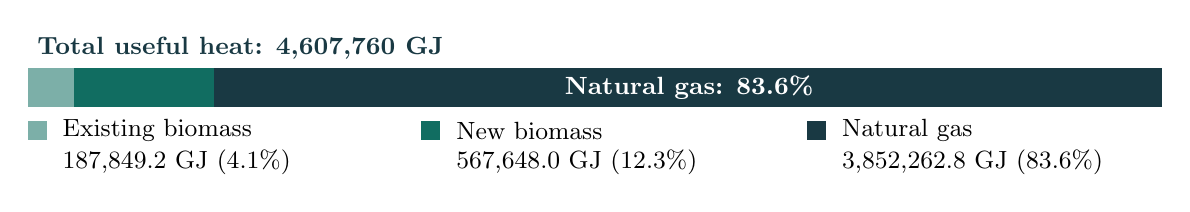
\begin{tikzpicture}[x=1cm,y=1cm,font=\small]
% Coordinates use the exported totals in TJ to keep PGF arithmetic in range.
\pgfmathsetmacro{\existingEnd}{14.4*(187.84917379957918/4607.76)}
\pgfmathsetmacro{\biomassEnd}{14.4*((187.84917379957918+567.648)/4607.76)}
\fill[accent!55] (0,0) rectangle (\existingEnd,0.50);
\fill[accent] (\existingEnd,0) rectangle (\biomassEnd,0.50);
\fill[ink] (\biomassEnd,0) rectangle (14.4,0.50);
\node[white,font=\small\bfseries] at (8.4,0.25) {Natural gas: 83.6\%};
\node[anchor=west,text=ink,font=\small\bfseries] at (0,0.75)
  {Total useful heat: 4,607,760 GJ};
\fill[accent!55] (0,-0.42) rectangle (0.24,-0.18);
\fill[accent] (5.0,-0.42) rectangle (5.24,-0.18);
\fill[ink] (9.9,-0.42) rectangle (10.14,-0.18);
\node[anchor=west] at (0.32,-0.30) {Existing biomass};
\node[anchor=west] at (5.32,-0.30) {New biomass};
\node[anchor=west] at (10.22,-0.30) {Natural gas};
\node[anchor=west] at (0.32,-0.70) {187,849.2 GJ (4.1\%)};
\node[anchor=west] at (5.32,-0.70) {567,648.0 GJ (12.3\%)};
\node[anchor=west] at (10.22,-0.70) {3,852,262.8 GJ (83.6\%)};
\end{tikzpicture}
\caption{Useful heat in the recorded 365-day GAMS-input baseline under the
corrected Python formulation. Source: \nolinkurl{results/phase4/gams-historical-inputs-365d/result.json}.
Bar widths use the saved annual heat totals. This is a time-limited,
audited feasible plan with a reported MIP gap of \(0.02890\%\).}
\label{fig:annual-heat}
\end{figure}

\section{Limitations and future research}
The demand profile, available plant capacity, silo layout, supply limits,
prices and factor bases require primary verification. Provisional emissions
are not a lifecycle assessment. Storage is evaluated at day end and assumes
no moisture change or material loss. The archival sensitivity plots lack
a reproducible run record and are not reused as validated results here.
Future work can establish verified inputs, tighten annual bounds, model
seasonal supply or receiving-time inventory, and generate cost--emissions
trade-offs by applying emissions ceilings to \eqref{eq:cost}. An
epsilon-constraint sweep should save matched outcomes, document gaps and
filter dominated solutions \cite{mavrotas2009}. This study does not
compute a Pareto frontier.

\section{Conclusions}
The corrected MILP can conserve fuel inventories, satisfy plant and demand
constraints, and reproduce independently established synthetic optima.
Storage and fuel-specific conversion can change the cheapest procurement
choice even in two days. Annual incumbents are reproducible evidence of
feasibility under stated assumptions. Confirming the historical inputs
and proving annual optimality are separate research tasks.

\bibliographystyle{unsrt}
\begingroup
\raggedright
\bibliography{references}
\endgroup

\appendix
\small
\section{Inventory and dimensional derivations}
The archived equations \texttt{co3} and \texttt{co4} equate the same
current closing stock to fresh receipts minus fresh burn, with prior stock
added in \texttt{co4}. Their difference leaves prior stock equal to zero.
Equation~\eqref{eq:stock} replaces both balances and subtracts withdrawals
from storage. The conversion in \eqref{eq:coefficient} uses
\(\mathrm{m^3}\times \mathrm{wet\ t/m^3}\times
\mathrm{dry\ t/wet\ t}\times\mathrm{GJ/dry\ t}\) times efficiency, giving
useful GJ. The archived emissions factor 0.5 is multiplied by three in the
gas sum because the same daily gas term appears for each \(f\). Equation
\eqref{eq:emissions} removes that repeated summation without selecting a
historically correct emissions factor.

\section{Hand enumeration for the two-plant fixtures}\label{app:enumeration}
The existing unit has 2 GJ/day; the new unit has 4 then 2 GJ. Each fuel
has 4 GJ of input energy per \(\mathrm{m^3}\). Useful coefficients
(existing, new) are chips \((2,3)\), pellets \((2,4)\), and briquettes
\((3,3)\). Truck volumes are 2, 2.5 and 2 \(\mathrm{m^3}\), at costs
2.40, 5.00 and 4.00, respectively. Gas costs 3 per GJ.
Table~\ref{tab:enum} lists all truck options. Chips can deliver 6 useful
GJ by storing \(2/3\,\mathrm{m^3}\) after day one. With no closing storage,
the remainder burns in the existing plant at lower efficiency, giving only
\(16/3\) GJ total. Briquettes supply 6 GJ on day one. Pellets need at least
\(0.5\,\mathrm{m^3}\) of first-day silo space to accept a full truck.

\begin{table}[htbp]
\small
\caption{Hand-calculated costs for each feasible day-one truck option.}
\label{tab:enum}
\begin{tabularx}{\textwidth}{@{}Yrrr@{}}
\toprule Choice & Base & Tighter silo & No storage\\ \midrule
No truck & 24.00 & 24.00 & 24.00\\
Chips & 8.40 & 8.40 & 10.40\\
Pellets & 5.00 & Infeasible & Infeasible\\
Briquettes & 10.00 & 10.00 & 10.00\\
\bottomrule
\end{tabularx}
\end{table}

\section{Reproducibility}
\textbf{Environment.} Install the versions in
\nolinkurl{requirements-phase2.txt}. Run from the repository root.

\medskip
\begin{lrbox}{\commandsbox}
\begin{minipage}{\dimexpr\linewidth-2\fboxsep\relax}
\vspace{4pt}
\begin{verbatim}
python -B -m unittest discover -s tests -v
python -B -m optimization.example
python -B -m optimization.example_phase3 --case base
python -B -m optimization.annual --scenario gams-historical-inputs
\end{verbatim}
\vspace{4pt}
\end{minipage}
\end{lrbox}
\noindent\colorbox{mist}{\usebox{\commandsbox}}

\medskip
\textbf{Scenario and solver controls.} Phase 3 also offers
\texttt{tight-silo} and \texttt{no-storage}. Add
\texttt{--time-limit 30} and \texttt{--output <folder>} to save the annual
JSON and CSV. The default is 30 seconds. A time-limited audited feasible
plan is exported before the CLI returns status 2.

\medskip
\textbf{Audit trail.} The inputs are in \nolinkurl{scenarios/annual.json}
and saved runs in \nolinkurl{results/phase4/}. Reproduce Figure~\ref{fig:annual-heat}
by summing \texttt{biomass\_gj\_by\_plant\_and\_fuel} by plant and
\texttt{gas\_gj} across the saved baseline days. The corrected MILP is in
\nolinkurl{optimization/phase3.py}, the unit and inventory checks in
\nolinkurl{validation/phase1.py}, and the horizon audit in
\nolinkurl{optimization/annual.py}.

\end{document}
